
%%%%%%%%%%%%%%%%%%%%%%%%%%%%%%%%%%%%%%%%%
% Short Sectioned Assignment
% LaTeX Template
% Version 1.0 (5/5/12)
%
% This template has been downloaded from:
% http://www.LaTeXTemplates.com
%
% Original author:
% Frits Wenneker (http://www.howtotex.com)
%
% License:
% CC BY-NC-SA 3.0 (http://creativecommons.org/licenses/by-nc-sa/3.0/)
%
%%%%%%%%%%%%%%%%%%%%%%%%%%%%%%%%%%%%%%%%%

\documentclass[paper=a4, fontsize=11pt]{scrartcl}
\usepackage[utf8]{inputenc}
\usepackage[spanish]{babel}
\usepackage{amsmath,amsfonts,amsthm}
\usepackage{sectsty}
\usepackage{fancyhdr}
\usepackage{sectsty}
\usepackage{graphicx}

\allsectionsfont{\textbf \normalfont}
\setlength\parindent{0pt}
\pagestyle{fancyplain}
\fancyhead{}
\fancyfoot[L]{Electrónica de Microondas}
\fancyfoot[C]{}
\fancyfoot[R]{\thepage}\fancyfoot[C]{}

\renewcommand{\headrulewidth}{0pt}
\renewcommand{\footrulewidth}{0pt}
\setlength{\headheight}{13.6pt}
\newcommand{\horrule}[1]{\rule{\linewidth}{#1}}
\newcommand{\exercisetitle}[1]{
\section{}
#1 \\[0.1cm]
\horrule{1pt}
}
\title{
\normalfont \normalsize
\huge Ejercicios Tema 3 \\
\horrule{2pt} \\[0.5cm]
}
\author{Luis Sánchez Velasco}
\date{\normalsize\today}

\begin{document}

\maketitle

\newcommand{\propconstant}[1]{
  \begin{equation*}
      \gamma = \sqrt{(R + j\omega L)(G + j \omega C)} #1
  \end{equation*}
}

\newcommand{\propconstantnoloss}[1]{
  \begin{equation*}
      \gamma =j\omega \sqrt{ L C} #1
  \end{equation*}
}

\newcommand{\impedance}[1]{
  \begin{equation*}
      Z_0 = \sqrt{\frac{(R + j\omega L)}{(G + j \omega C)}}  #1
  \end{equation*}
}

\newcommand{\impedancenoloss}[1]{
  \begin{equation*}
    Z_0 = \sqrt{\frac{L}{C}} #1
  \end{equation*}
}

\newcommand{\swr}[1]{
  \begin{equation*}
    SWR = \frac{1 + | \Gamma_L |}{1 - | \Gamma_L |} #1
  \end{equation*}

}

\exercisetitle{
Una línea de transmisión posee los siguientes parámetros por unidad de longitud: $L=0.3\mu H/m$, $C=450pF/m$,
$R=5\Omega /m$, y $G=0.01S/m$. Calcular la constante de propagación y la impedancia característica de esta
línea a $880MHz$. Recalcular estos parámetros en ausencia de pérdidas.}

La constante de propagación en medios con perdidas se define como:
\propconstant{ = \alpha + j \beta}
Donde sustituyendo por los valores dados en el ejercicio, $L=0.3\mu H/m$, $C=450pF/m$, $R=5\ohm /m$, y $G=0.01S/m$ obtenemos:
\begin{align*}
  \alpha &= 0.226 \\
    \beta &= 64.2
\end{align*}
Y para el cálculo de la impedancia característica:
\impedance{= 25.8 + 0.01j }
\\[0.5cm]
Para el caso sin perdidas asumiremos $R = G= 0$, por lo que la constante de propagación quedará como:
\propconstantnoloss{ = 64j}
y la impedancia característica:
\impedancenoloss{= 25.8 \Omega}

\exercisetitle{
Una línea de transmisión sin perdidas de longitud $0.3\lambda$ termina en una impedancia de carga, $Z_L$. Encontrar
el coeficiente de reflexión en la carga, el SWR de la linea y la impedancia de entrada de la linea. $(Z_0=75
\Omega, Z_L = 40 + j20 \Omega)$.
}
Para calcular primeramente el coeficiente de reflexión, situaremos en la carta de Smith el punto $z = \frac{40}{75} + \frac{20}{75}j \Omega$, marcado con un '1' en al gráfica. Donde observando el ángulo y la fase de este punto, obtenemos:
\[ \Gamma_L = 0.34e^{j2.45} \]

Para calcular el SWR haremos:
\swr{ \approx 2}

Para calcular la impedancia a la entrada moveremos el punto '1' $0.3 \lambda$ hacia el generador, punto '2' y observaremos que lineas corta. En este caso:
$z_i = 0.94 + 0.7i$ que al denormalizar quedará como: $Z_{in} = 67.5 + 52.5j$.

\begin{figure}[h]
  \centering
  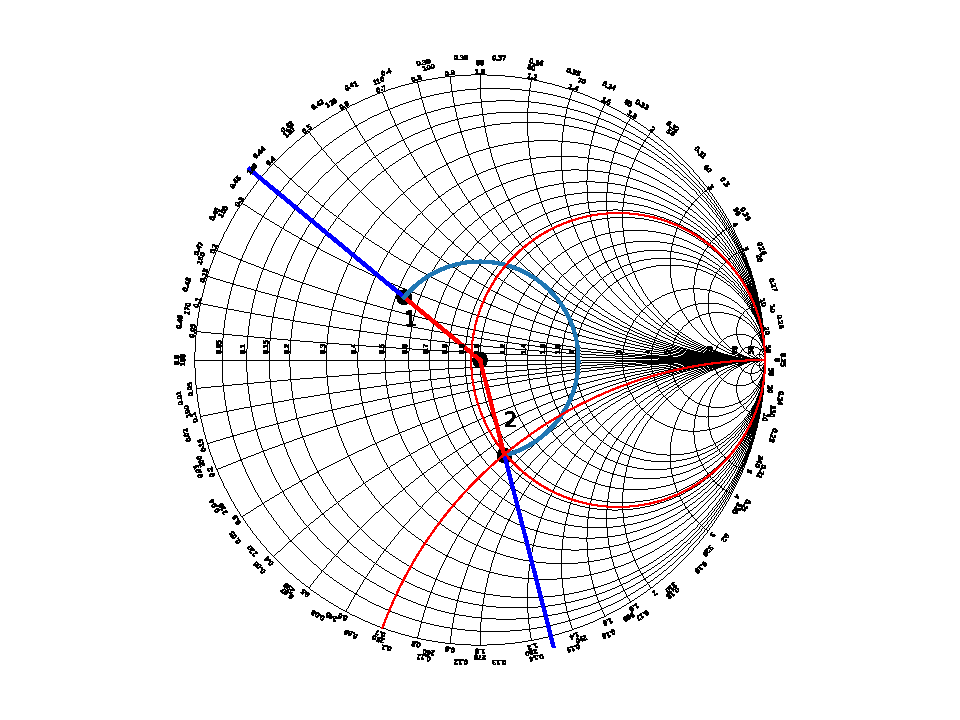
\includegraphics[scale = 0.85]{ej2/images/out.pdf}
  \caption{Moviendo el punto $0.3 \lambda$}
  \label{ej2smith}
\end{figure}

\exercisetitle{
Una línea de transmisión sin pérdidas de impedancia característica $Z_0$ se termina con una impedancia de
carga de $150 \Omega$.  Si se mide una SWR en la línea de 1.6, encontrar los dos posibles valores para $Z_0$.
}
Aunque el enunciado nos dice que existen dos posible valor para $Z_0$, solo existe uno, ya que tanto la impedancia de carga, como la de la línea (sin pérdidas), son reales.
Para resolverlo empezaremos evaluando la expresión del SWR:
\swr{ = 1.6}
Donde podemos resolver para $| \Gamma_L |$,obteniendo:
\[ | \Gamma_L | = 0.23 \]
Sabemos que al ser las dos impedancias puramente reales, el valor absoluto del coeficiente de reflexión será igual a su valor real, esto se puede observar en la expresión del coeficiente de reflexión en función de la impedancia de carga y la impedancia carcterística de la línea.

\reflectionfromimpedance{ = 0.23}

De donde podemos obtener $Z_0$, el cual resulta:
\[Z_0 = 93.9 \Omega \]

\end{document}
